\documentclass[10pt,conference]{IEEEtran}
\IEEEoverridecommandlockouts
% The preceding line is only needed to identify funding in the first footnote. If that is unneeded, please comment it out.
\usepackage{cite}
\usepackage{amsmath,amssymb,amsfonts}
\usepackage{algorithmic}
\usepackage{graphicx}
\usepackage{textcomp}
\usepackage{booktabs}
\usepackage[table,xcdraw]{xcolor}
\usepackage{framed}
\usepackage{float}
\usepackage{xcolor}

\usepackage{xfrac}

\usepackage{balance}

\usepackage{array}
\newcolumntype{L}[1]{>{\raggedright\let\newline\\\arraybackslash\hspace{0pt}}m{#1}}


\usepackage{listings}

\definecolor{mygreen}{rgb}{0,0.6,0}
\definecolor{lightgreen}{rgb}{0.6,0.9,0.6}
\definecolor{lightyellow}{rgb}{0.9,0.9,0.6}
\definecolor{lightorange}{rgb}{0.9,0.8,0.6}
\definecolor{lightred}{rgb}{0.9,0.7,0.7}
\definecolor{mygray}{rgb}{0.5,0.5,0.5}
\definecolor{lightgray}{rgb}{0.8,0.8,0.8}
\definecolor{mymauve}{rgb}{0.58,0,0.82}


\usepackage{pifont}
\newcommand{\lstbg}[3][0pt]{{\fboxsep#1\colorbox{#2}{\strut #3}}}
\lstset{ %
  language=C,
  backgroundcolor=\color{white},   % choose the background color
  basicstyle=\ttfamily\scriptsize,        % size of fonts used for the code
  breaklines=true,                 % automatic line breaking only at whitespace
  captionpos=b,                    % sets the caption-position to bottom
  commentstyle=\color{mygray}\bfseries,    % comment style
  escapeinside={\%*}{*)},          % if you want to add LaTeX within your code
  keywordstyle=\color{blue},       % keyword style
  stringstyle=\color{mymauve},     % string literal style
  frame=single,
  numbers=left,
  stepnumber=1,
  xleftmargin=2em,
  escapeinside={/*!}{!*/},
  moredelim=**[l][\color{mygreen}]{+\ },
  moredelim=*[l][\color{red}]{-\ }
}


\newcounter{lstannotation}
\setcounter{lstannotation}{0}
\renewcommand{\thelstannotation}{\ding{\number\numexpr181+\arabic{lstannotation}}}
\newcommand{\annotation}[1]{\refstepcounter{lstannotation}\label{#1}\thelstannotation}


\def\BibTeX{{\rm B\kern-.05em{\sc i\kern-.025em b}\kern-.08em
    T\kern-.1667em\lower.7ex\hbox{E}\kern-.125emX}}

\newcommand{\Sof}[1]{\textbf{[Sofia:[}{\color{red} #1}\textbf{]]}}


\begin{document}

\title{Fixing Vulnerabilities Hinders Maintainability}

\author{
    Anonymou(s) Author(s)
%     \IEEEauthorblockN{1\textsuperscript{st} Given Name Surname}
% \IEEEauthorblockA{\textit{dept. name of organization (of Aff.)} \\
% \textit{name of organization (of Aff.)}\\
% City, Country \\
% email address}
% \and
% \IEEEauthorblockN{2\textsuperscript{nd} Given Name Surname}
% \IEEEauthorblockA{\textit{dept. name of organization (of Aff.)} \\
% \textit{name of organization (of Aff.)}\\
% City, Country \\
% email address}
% \and
% \IEEEauthorblockN{3\textsuperscript{rd} Given Name Surname}
% \IEEEauthorblockA{\textit{dept. name of organization (of Aff.)} \\
% \textit{name of organization (of Aff.)}\\
% City, Country \\
% email address}
}

\maketitle

\begin{abstract}
Security is a requirement of utmost importance to produce software with high
quality. However, there is still a considerable amount of zero-day
vulnerabilities being discovered, and fixed, almost weekly. We suspect that when
developers address these vulnerabilities on their codebases, they actually
affect the maintainability of software, potentially introducing other
vulnerabilities. This paper evaluates the impact of refactorings to improve
security on the maintainability of open-source software. Maintainability is
measured based on the \emph{Better Code Hub}'s model of 10 guidelines using a
dataset including $607$ security commits. Results show that fixing software
vulnerabilities hinders the maintainability of open-source software. This is
particularly the case for refactorings that address \emph{Broken Authentication
and Session Management} issues, \emph{Memory Leaks} and \emph{Denial-of-Service}
attacks. Furthermore, we conclude that changes to codebases to fix vulnerabilities
need to be performed with extra care.
\end{abstract}

\begin{IEEEkeywords}
Security, Software Maintenance, Open-Source Software
\end{IEEEkeywords}

\section{Introduction}

Software quality is important because it is ultimately related to the overall
cost for developing, extending and maintaing software applications. Software
quality characteristics include, but are not limited to, functional correctness,
reliability, usability, maintainability, and security. Security is an important
non-functional requirement during the development of software systems.  However,
there is still a considerable amount of zero-day vulnerabilities being
discovered, and fixed, almost weekly as disclosed by the Zero Day Initiative
website\footnote{Zero Day Initiative website available  at
https://www.zerodayinitiative.com/advisories/published/ (Accessed on \today{})}.
As an example, in the last week of January 2019, a severe vulnerability in Apple
FaceTime was
revealed\footnote{https://thehackernews.com/2019/01/apple-facetime-privacy-hack.html
(Accessed on \today{})}. Callers could see and hear others without them picking up the call. These vulnerabilities are gateways for attackers to
penetrate systems and exploit their resources. 

\Sof{Models} Lorem Ipsum is simply dummy text of the printing and typesetting industry. Lorem Ipsum has been the industry's standard dummy text ever since the 1500s, when an unknown printer took a galley of type and scrambled it to make a type specimen book. It has survived not only five centuries, but also the leap into electronic typesetting, remaining essentially unchanged. It was popularised in the 1960s with the release of Letraset sheets containing Lorem Ipsum passages, and more recently with desktop publishing software like Aldus PageMaker including versions. 


In 2011, the International Organization for Standardization (ISO) issued an
update for software product quality ISO/IEC 25010~\cite{iso:2011} considering
\emph{Security} as one of the main software product quality characteristics.
Unmaintainable code is hard to test, analyse and re-use, and thus more difficult
to find vulnerabilities and defects. Therefore, writing maitainable code
prevents the introduction of vulnerabilities in the code. In this work, we are
concerned about the impact that fixing vulnerabilities may have in the
maintainability of open-source software. Are developers affecting software
maintainability when trying to improve software safety? We suspect that some of
those fixes may have a negative impact in the software maintainability and
possibly even be the cause of the introduction of new vulnerabilities.

ISO describes software maintainability as ``the degree of effectiveness and
efficiency with which a software product or system can be modified to improve
it, correct it or adapt it to changes in environment, and in requirements'' on
software quality ISO/IEC 25010. As ISO does not provide any specific guidelines or
formula to calculate maintainability, we resort on Software Improvement
Group (SIG)’s web-based source code analysis service Better Code Hub
(BCH)~\cite{Visser:2016:OREILLY} to compute the maintainability of a given
project. BCH compiles the ISO/IEC 25010 into a set of 10 guidelines that are the
base of BCH's evaluation. Two examples of guidelines used by BCH are the
\emph{Write Simple Units of Code} based on the McCabe Complexity~\cite{1702388}
and \emph{Keep your Codebase Small} based on the idea that smaller codebases are
easier to maintain and less sensitive to defects~\cite{Visser:2016:OREILLY}.
Compliance to the guidelines is derived from the SIG's
industry benchmark which, according to official sources, consists of over 8
billion lines of code in more than 180 different technologies. SIG analyzes
around 15 million lines of code, per week.

The particular subject of this paper is to explore whether there is a trade-off
between refactoring source code to fix identified vulnerabilities while keeping
(or even improving) the maintainability of the software system. In other words,
we are interested in answering the following overarching question

\begin{framed}
\noindent
Does improving security have a negative impact on code
maintainability?
\end{framed}

\noindent
In this paper, we present the results of our analysis on the maintainability of
607 security changes collected from open-source software, from different
programming languages.

The main contributions of the present work is:
\begin{itemize}
	\item An empirical study on the impact of security changes on software
	maintainability and what patterns need more attention.

  % \item An analysis of how likely security-related changes need to be
  % maintained, in comparison to regular commits.

	\item A replication package with all scripts and data created to perform the
	empirical evaluation, for reproducibility. Available here: $<url>$.

\end{itemize}

This empirical study exhibits proof that changes applied in the codebase to fix
vulnerabilities affect code maintainability. Especially, for refactorings that
address \emph{Broken Authentication and Session Management} issues, \emph{Memory
Leaks} and \emph{Denial-of-Service} attacks. With this study, we intend to
highlight the need for tools and documentation to help developers adopt security
best practices.

This paper is structured as follows: section \ref{sec:motivation} introduces an
example of a security refactoring of a known vulnerability found in
OpenSSL\footnote{Repository available at https://github.com/openssl/openssl
(Accessed on \today{})} software; section \ref{sec:methodology} describes the
methodology used to answer the research questions; section \ref{sec:results}
presents the results and section \ref{sec:discussion} discusses their
implications; section \ref{sec:threats}, threats to the validity of the study
are enumerated; section \ref{sec:rw} describres the different work and existing
literature in the field of study; and, finally section \ref{sec:conclusions}
concludes the main findings and elaborates on future work.
%
\section{Motivation and Research Questions}\label{sec:motivation}
%
Due to time-to-market pressure and the lack of security expertise, code-related
security flaws are generally detected \textit{after the fact}, i.e., when
hackers exploit them. It turns out that fixing these issues is as simple as
modifying the software codebase. However, these refactorings may have a negative
impact on software maintenance, mostly because developers follow the quickest
solution to fix the problem and not necessarily the most elegant and performant
one. Thus, we want to understand how security refactorings impact the
maintainability of software.

As an example, consider the refactoring of the Datagram Transport Layer Security
(DTLS) protocol implementation in OpenSSL to address the fact that hackers could
cause a Denial-of-Service (DoS) attack by crafting DTLS
handshake messages to trigger memory allocations corresponding to large length
values. This vulnerability is listed at the Common Vulnerabilities and Exposures
dictionary as CVE-2014-3506\footnote{CVE-2014-3506 details available at
http://cve.mitre.org/cgi-bin/cvename.cgi?name=CVE-2014-3506 (Accessed on
\today{})}. It is amongst the vulnerabilities studied in our evaluation.
The following snippet presents the changes performend on the
\emph{ssl/d1\_both.c} file\footnote{CVE-2014-3506 fix available  at
https://github.com/openssl/openssl/commit/\\1250f12613b61758675848f6600ebd914ccd7636
(Accessed on \today{})} by the OpenSLL developers to fix the vulnerability.


\setcounter{lstannotation}{0}
\begin{lstlisting}[caption={Fix provided by OpenSSL developers to the
\\CVE-2014-3506 vulnerability},label={lst:vuln}]
+ static unsigned long dtls1_max_handshake_message_len(const SSL *s){ /*!\annotation{lst:func1}!*/
+  unsigned long max_len = DTLS1_HM_HEADER_LENGTH + SSL3_RT_MAX_ENCRYPTED_LENGTH;
+  if(max_len < (unsigned long)s->max_cert_list) /*!\annotation{lst:func2}!*/
+     return s->max_cert_list;
+  return max_len;
+ }

  static int dtls1_reassemble_fragment(SSL *s, struct hm_header_st* msg_hdr, int *ok){

// [snip]

- unsigned long frag_len = msg_hdr->frag_len, max_len; /*!\annotation{lst:func3}!*/
- if((msg_hdr->frag_off+frag_len) > msg_hdr->msg_len)
-    goto err;

- if(DTLS1_HM_HEADER_LENGTH +
-    	SSL3_RT_MAX_ENCRYPTED_LENGTH < s->max_cert_list)
-    max_len = s->max_cert_list;
- else
-    max_len = DTLS1_HM_HEADER_LENGTH +
-   		SSL3_RT_MAX_ENCRYPTED_LENGTH;

+ unsigned long frag_len = msg_hdr->frag_len;

- if((msg_hdr->frag_off+frag_len) > max_len)

+ if((msg_hdr->frag_off+frag_len) > msg_hdr->msg_len ||
+ msg_hdr->msg_len > dtls1_max_handshake_message_len(s))
     goto err; /*!\annotation{lst:func5}!*/

  memset(seq64be,0,sizeof(seq64be));
  seq64be[6] = (unsigned char) (msg_hdr->seq>>8);
  seq64be[7] = (unsigned char) msg_hdr->seq;
  item = pqueue_find(s->d1->buffered_messages, seq64be);
  if(item == NULL)
  {
    frag = dtls1_hm_fragment_new(msg_hdr->msg_len, 1);

// [snip]

 static int
 dtls1_process_out_of_seq_message(SSL *s, struct hm_header_st* msg_hdr, int *ok)
 {

// [snip]

  if(frag_len && frag_len < msg_hdr->msg_len)
     return dtls1_reassemble_fragment(s, msg_hdr, ok);

+ if(frag_len > dtls1_max_handshake_message_len(s))
+    goto err; /*!\annotation{lst:func4}!*/
+
  frag = dtls1_hm_fragment_new(frag_len, 0);

\end{lstlisting}

In the \texttt{dtls1\_reassemble\_fragment} function the value of
\texttt{msg\_hdr-$>$frag\_off+frag\_len} is checked against the maximum
handshake message size, but \texttt{msg\_len} is allocated to the fragment
buffer in line $37$. Thus, if the fragment was within the allowed size, the
pending handshake message could consume $18MB$ ($16MB$+$2MB$). According to the
message commit, $10$ handshake messages are allowed, so the attacker could
consume approximately $180MB$ per DTLS connection.

The code changes performed to fix the vulnerability were the following:

\ref{lst:func1} \texttt{dtls1\_max\_handshake\_message\_len} function was
inserted to limit the number of bytes allowed in a DTLS handshake message for
\texttt{s}. This function replaces lines $18$---$21$.

\ref{lst:func2} Checks if the maximum certificate list size
(\texttt{s-$>$max\_cert\_list}) requires more length than the maximum length
(\texttt{max\_len}). If yes, it return the certificate list size, if not it
return the maximum length.

\ref{lst:func3} Replaced by attribution in line $23$.

\ref{lst:func5} and \ref{lst:func4} add the check to ensure that the message
length is never higher than the maxiumum allowed by the DTSL protocol in
different functions.

Although limiting the size of a handshake message seems an elementary problem to
repair, the example shows that there was a significant amount of changes
performed in the codebase which produced a negative impact in the project
maintainability. Even though the developer tries to simplify the codebase with
the creation of a smaller unit \texttt{dtls1\_max\_handshake\_message\_len}, it
also disrupts $2$ of the guidelines proposed by the Software Improvement Group
(SIG) for building maintainable software~\cite{Visser:2016:OREILLY}. It adds a
new branch point to the \texttt{dtls1\_process\_out\_of\_seq\_message} unit
(\ref{lst:func5}) increasing the cyclomatic complexity and breaking the
\emph{Write Simple Units of Code} guideline. And, it increases the codebase size
in $4$ lines of code ($13$ lines added, $9$ lines deleted) which infringes the
\emph{Keep Your Codebase Small} guideline. Hence, we have observed that the
impact of this refactoring on the OpenSSL maintainability was negative.

In this study, our concern is to study whether while improving software
security, developers are also inserting a negative impact on the maintainability
of their software which may increase technical debt when choosing the easiest
solution instead of the using the best approach. To answer the following two
research questions, we use a dataset of security refactorings to measure the
impact of the changes in the maintainability of open-source software.

\begin{framed}
\textit{\textbf{RQ1} What is the impact of security refactorings on the
maintainability of open-source software?}
\end{framed}

Often security flaws require refactoring code to make software more secure.
However, there is no evidence yet of how security refactorings impact the
maintainability of open-source software. Our suspicion is that developers tend
to introduce technical debt in their software when refactoring the codebose to
address a security flaw because they tend to choose the easiest path to solve
it. To address it, we compute the maintainability value of $607$ commits using
\emph{Better Code Hub}. The same approach is applied to a randomly generated
dataset of regular commits - baseline - that we use to understand how
maintainability evolves when security refactorings are performed versus when
they are not.

\begin{framed}
\textit{\textbf{RQ2} Which patterns of security refactorings are more likely to
affect open-source software maintainability?}
\end{framed}

There are security flaws that are more difficult to refactor than others. For
instance, introducing a mechanism to secure authentication is not so easy to
implement as fixing a cross-site scripting vulnerability with a \texttt{escape}
function. Knowing which patterns are more likely to increase maintainability
issues is one step forward to bring awareness to security engineers of what
patterns need more attention. The taxonomy of security patterns used to answer
this question is the same as the one provided by the authors of the dataset.
Maintainability is measured separately for each pattern.
%
\section{Methodology}\label{sec:methodology}
%
The methodology used to measure the impact of security refactorings on the
maintainability of open-source software is discussed in the following sections
and illustrated in Figure \ref{fig:met}. Aiming to answer the research questions
outlined in the previous section, in this paper, we use a dataset containing
$716$ security refactorings collected from open-source software available on
GitHub~\cite{Reis:2017:IJSSE}. Moreover, a baseline of regular commits was
randomly collected from the list of projects of the main dataset to evaluate
what is the impact of regular commits on the maintainability of open-source
software. The Software Improvement Group's\footnote{SIG's website is available
at https://www.sig.eu/ (Accessed on \today{})} web-based source code analysis
service \emph{Better Code Hub} (BCH)\footnote{BCH's website is available at
https://bettercodehub.com/ (Accessed on \today{})} was used to quantify
maintainability for both security and regular commits.
%
\begin{figure}[h]
 	\centering 	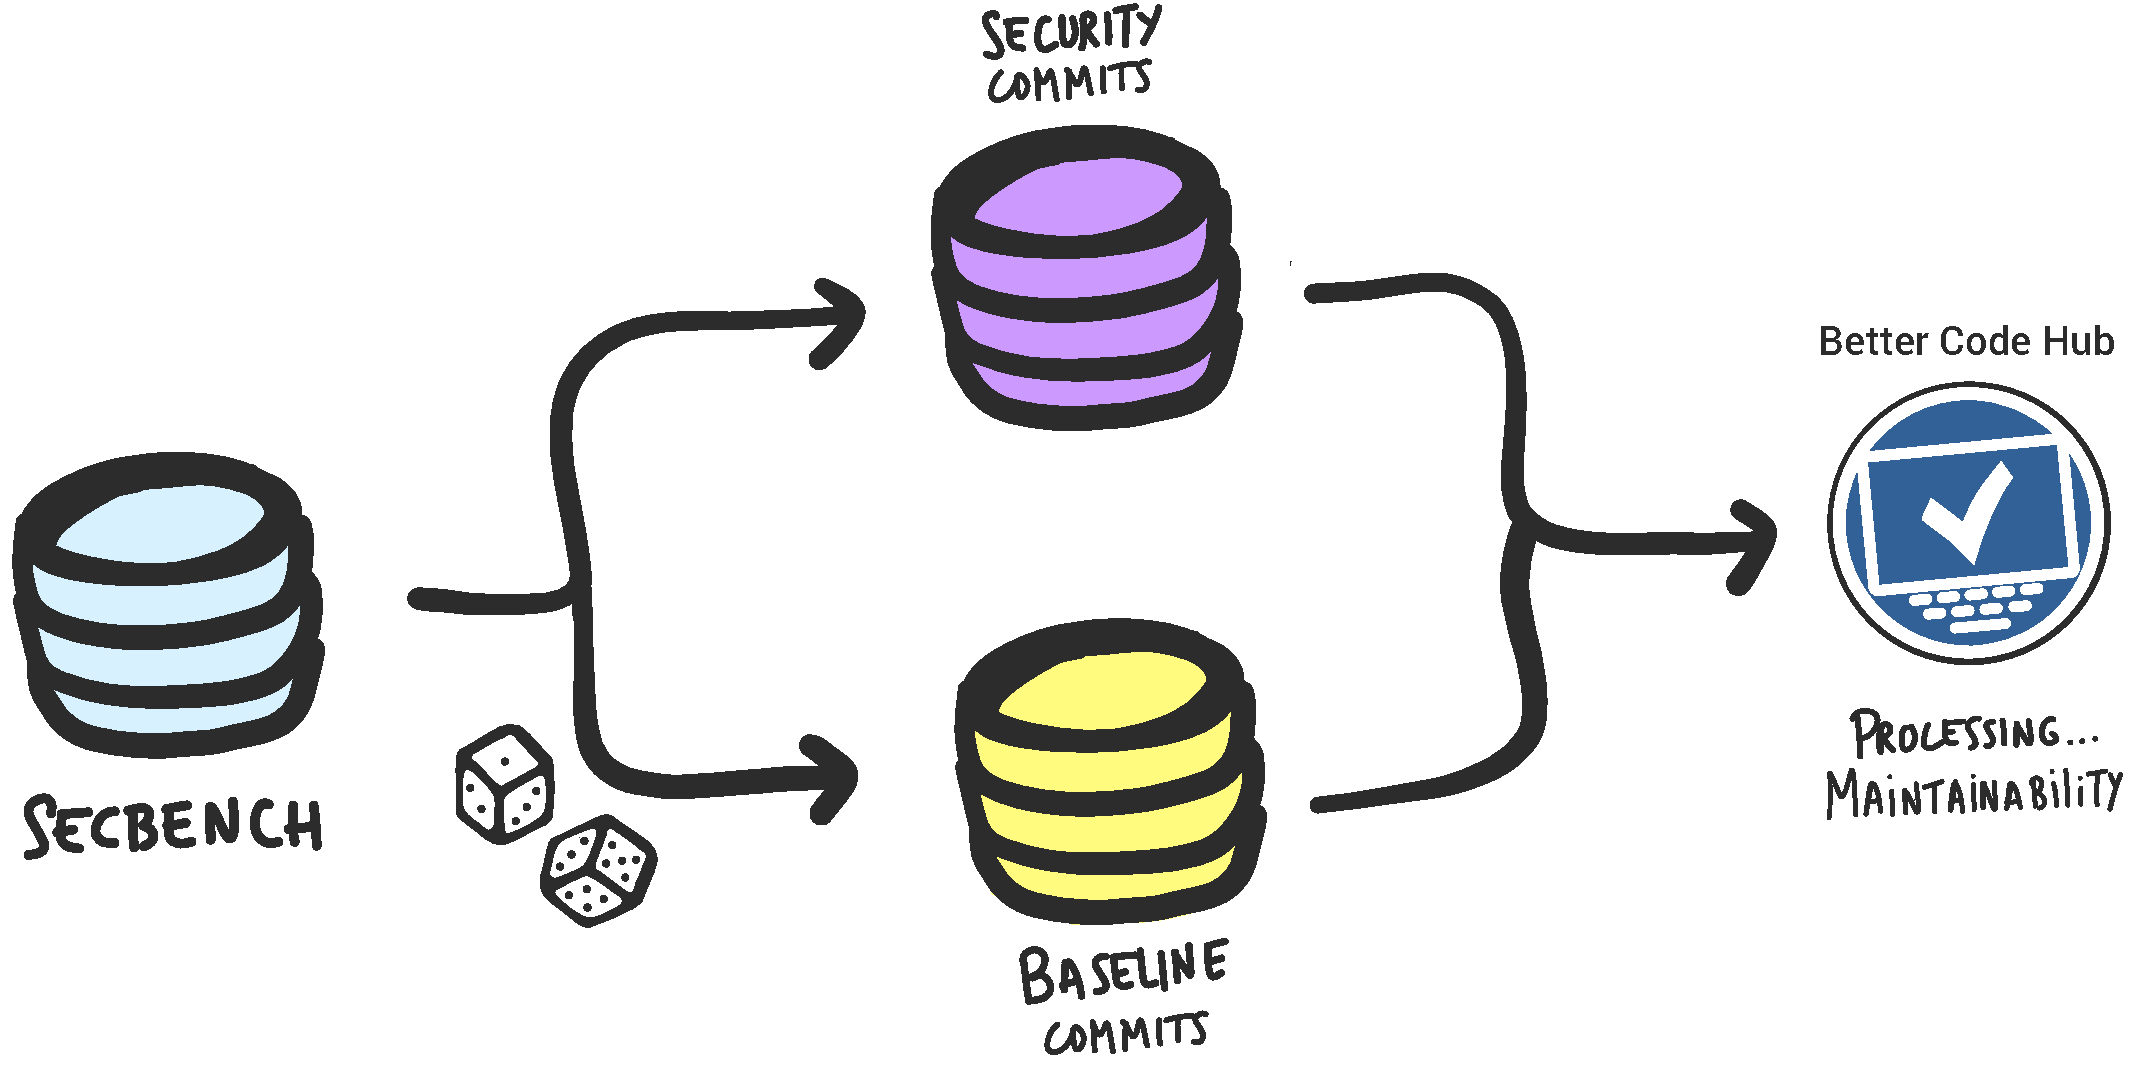
\includegraphics[width=0.5\textwidth]{figures/methodology.pdf}
 	\caption{Study Methodology}
	\label{fig:met}
\end{figure}
%
\subsection{Dataset}
%
To evaluate the impact of security refactorings on the maintainability of
open-source software, we use a dataset of security flaws which is the outcome of
mining $94$ GitHub projects. Reis and Abreu (2017) mined open-source
software aiming at the extraction of real examples --- created by real
developers --- to test and assess the performance of static analysis tools since
using hand-seeded test cases or mutations could lead to misleading assessments
of the capabilities of the tools \cite{just2014mutants}. The study yielded a
dataset with $716$ test case for $16$ security patterns. Each test case of the
dataset is a triplet: the commit before the refactoring, the commit responsible
for the refactoring and the snippets of code that differ from one version to
another (typically, called \textit{diff}) --- where one can easily identify the
code used to fix the security flaw. In this study, we focus on computing the
maintainability of the commits before and after the security refactoring to
evaluate if the impact was positive, negative or none.

\begin{figure}[h]
 	\centering 	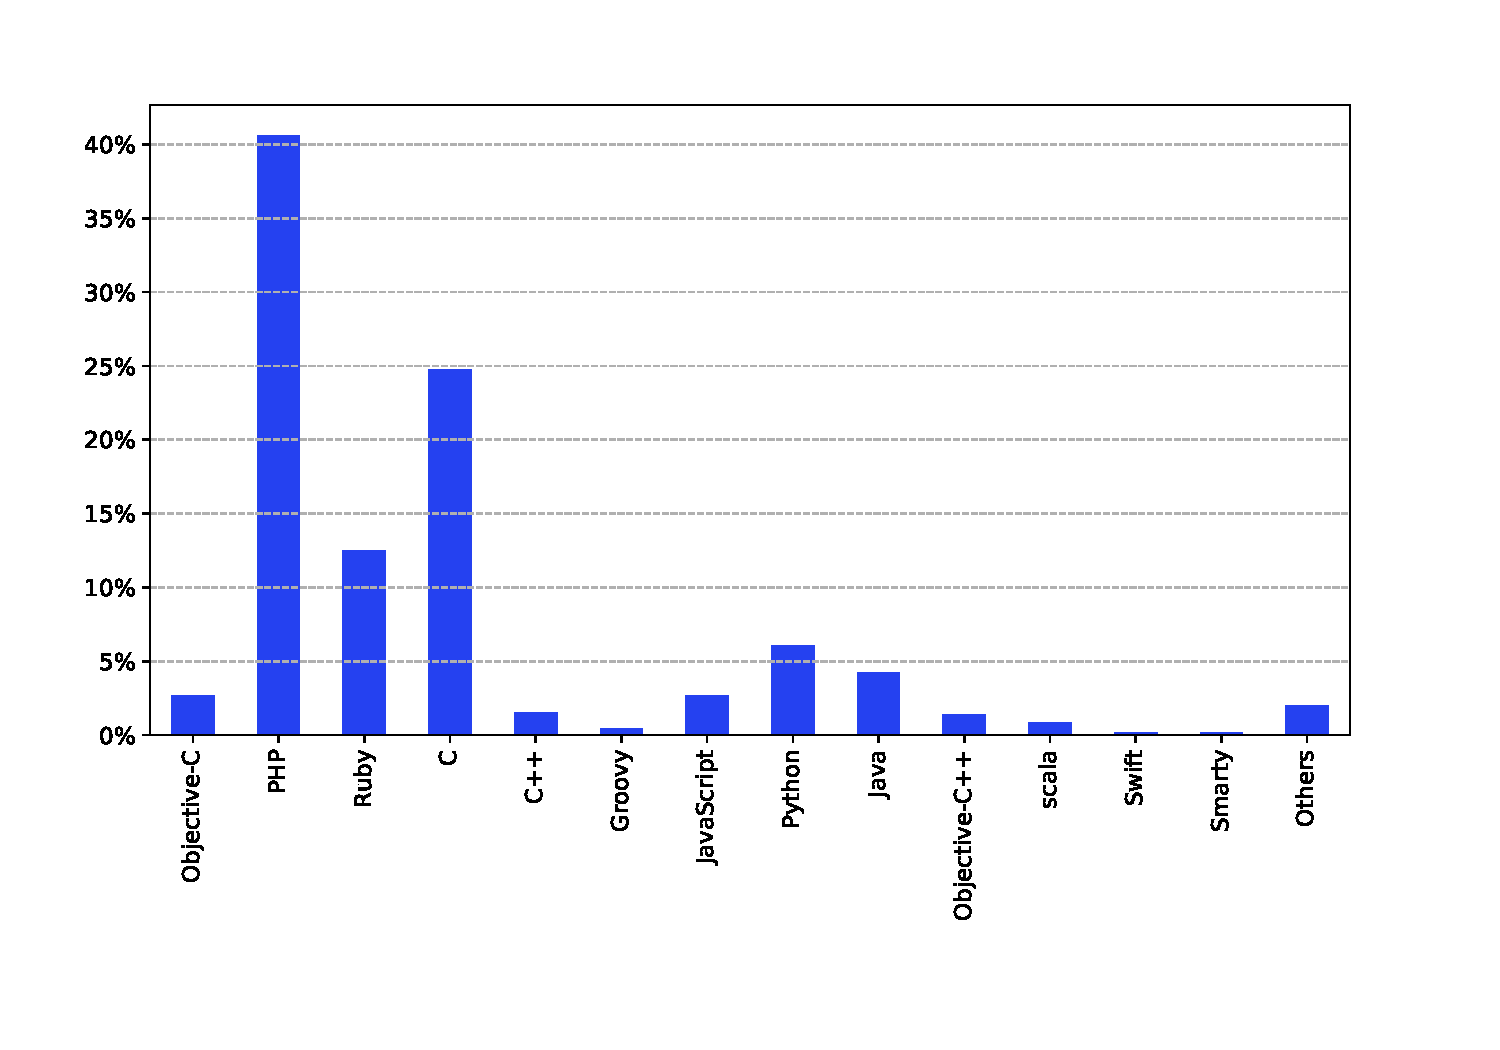
\includegraphics[width=0.5\textwidth]{figures/language_dist.pdf}
 	\caption{Security Refactorings Language Distribution}
	\label{fig:lang}
\end{figure}

\begin{figure}[h]
 	\centering 	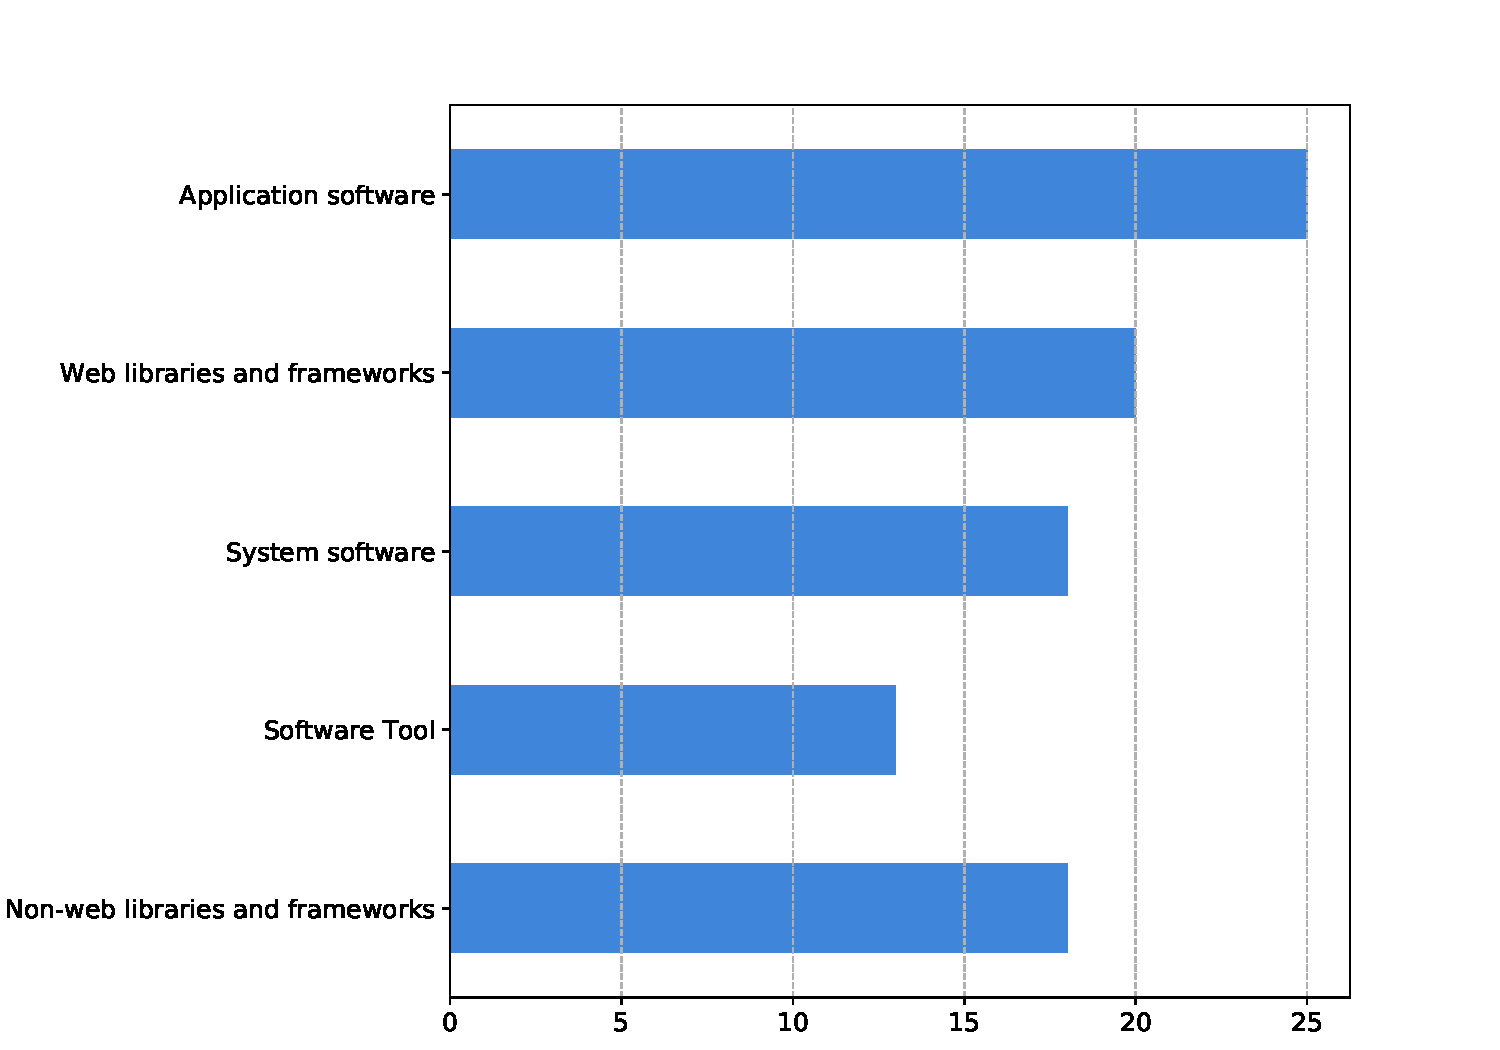
\includegraphics[width=0.5\textwidth]{figures/type_dist.pdf}
 	\caption{Projects Domain Distribution}
	\label{fig:domain}
\end{figure}

The test cases in the dataset are classified with one of the $16$ following
patterns, as based in the OWASP Top 10 of 2013~\cite{oswap:2013} and OWASP Top
10 of 2017~\cite{oswap:2017}: \textit{Injection}, \textit{Broken Authentication
and Session Management}, \textit{Cross-Site Scripting}, \textit{Broken Access
Control}, \textit{Security Misconfiguration}, \textit{Sensitive Data Exposure},
\textit{Insufficient Attack Protection}, \textit{Cross-Site Request Forgery},
\textit{Using Components With Known Vulnerabilities}, \textit{Unprotected APIs},
\textit{Memory Leak}, \textit{Overflow}, \textit{Denial-of-Service},
\textit{Path Traversal}, \textit{Miscellaneous}, \textit{Resource Leak} and
\textit{SHA-1 Hash Function}.

The $716$ refactorings in the dataset were run against the BCH toolset to
calculate their maintainability reports. However, there are refactorings
discarded from tour study due to limitations of BCH: in particular, lack of
language support and project size. The final dataset used in this paper contains
$607$ security refactorings, labelled as one of the following categories (we
have decided to change the label to \textit{Miscellaneous} of the patterns in
the dataset containing less than $20$ instances):

\begin{itemize}
	\item \textbf{Using Components with Known Vulnerabilities.} The majority of
	software produced today integrates several components, such as libraries and
	frameworks, which may affect the software if developers use vulnerable
	versions - usually known and disclosed somewhere on the Internet.
	\textit{Based on the OWASP Top 10 of 2017.}

	\item \textbf{Broken Authentication \& Session Management.} Uncorrectly
	implemented functionalities related to authentication and session management,
	allowing crackers to gain access to session tokens, passwords, keys and other
	sensitive data. \textit{Based on the OWASP Top 10 of 2013.}

	\item \textbf{Cross-Site Request Forgery.} Poor session tokens generation and
	management usually allow crackers to send forged HTTP requests including
	authentication information from the victim to vulnerable web application.
	\textit{Based on the OWASP Top 10 of 2013.}

	\item \textbf{Denial-of-Service} Security flaws that can allow a cracker to
	flood or crashing services. This attacks usually occur when the system
	receives much traffic causing it to slow down and eventually stop. For
	example, flaws allowing crackers to trigger memory allocations corresponding
	to large length values (Listing \ref{lst:vuln}).

	\item \textbf{Miscellaneous} This pattern comprises several others categories
	of security refactorings (e.g., \textit{path traversal and buffer overflow}).
	It contains several other security refactorings that do not have their own
	pattern yet. The patterns not satisfying the size requirement of more than 20
	refactorings are contemplated here.

	\item \textbf{Cross-Site Scripting.} Lack of proper validation or escaping
	allow crackers to submit untrusted data to web browsers through malicious
	scripts that can hijack the user sessions or redirect the user to malicious
	sites. \textit{Based on the OWASP Top 10 of 2017.}

	\item \textbf{Injection.} When developers do not keep untrusted data separate
	from commands and queries. If a cracker sends a string that exploits the
	syntax of the interpreter, then an injection attack is possible (e.g., SQL and
	LDAP injection). \textit{Based on the OWASP Top 10 of 2017.}

	\item \textbf{Memory Leak.} Memory management issue found more frequently in
	programming languages that do not manage memory automatically (e.g., C/C++ and
	Objective-C), i.e., where instead developers are responsible for handling it.
	One of the main causes of DoS attacks.
\end{itemize}

\begin{table*}[h]
	\centering
	\caption{Descriptive statistics of the dataset projects}
\begin{tabular}{@{}lllllllllll@{}}
\toprule
      & Forks   & Stars   & Watchers & Contributors & Commits  & Branches & Releases & Size      & Issues & Pull Requests  \\ \midrule
mean  & 1763.52 & 5448.74 & 401.37   & 153.33       & 14834.17 & 45.17    & 129.45   & 122973.24 & 3768.97   & 1941.61 \\
std   & 2434.03 & 6215.09 & 486.60   & 123.68       & 22234.46 & 150.15   & 189.93   & 209732.51 & 5933.16   & 3603.31 \\
min   & 1       & 3       & 1        & 0            & 103      & 1        & 0        & 108       & 0         & 0       \\
25\%  & 391.50  & 1581    & 117.25   & 49           & 1440.50  & 4        & 19       & 8466.75   & 313.75    & 143.25  \\
median  & 838.50  & 2836.50 & 248      & 99           & 5504.50  & 9        & 59       & 37372.50  & 1792.50   & 650     \\
75\%  & 2155    & 6828.50 & 459.50   & 261          & 18579.25 & 20       & 142.75   & 117699.50 & 4087.75   & 1907.25 \\
max   & 16366   & 31841   & 3446     & 413          & 114378   & 1227     & 1114     & 995790    & 33970     & 19329   \\
Total & 165771  & 512182  & 37729    & 14413        & 1394412  & 4246     & 12168    & 11559485  & 354283    & 182511  \\ \bottomrule
\end{tabular}
\label{tab:dataset}
\end{table*}

The dataset contemplates security flaws for more than 13 different languages
being PHP (39\%) and C (24\%) the most prevalent ones; see Figure \ref{fig:lang}.
To classify the applications in the dataset, we use a taxonomy for open-source
software published in an older study~\cite{7816479}. Figure \ref{fig:domain}
presents the projects domain distribution: \textit{Aplication Software} ($25$),
software that provides end-users with functional systems; \textit{Web libraries
and frameworks} ($20$); \textit{System Software} ($18$), software that provides
services and infrustructures (e.g., operating systems, servers and databases);
\textit{Software Tool} ($13$), software that supports development (e.g.,
programming languages, compilers, package managers, IDEs); and, \textit{Non-web
libraries and frameworks} ($18$), for desktop and mobile software.
%
Table \ref{tab:dataset} presents the descriptive statistics of the $94$
open-source projects involved in this study, icluding number of forks, number of
stars, number of watchers, number of contributors, number of commits, number of
branches, number of releases,  size (cf. GitHub it is the size of the whole
repository, including all of its history, in kilobytes), number of issues and pull
requests.


%
\subsection{Security vs. Baseline Commits}
%
Previous studies attempted to measure the impact of code refactorings on
open-source software maintainability~\cite{HEGEDUS2018313} before. But, to the
best of our knowledge, no previous work has used the BCH model and focused on
evaluating the impact of security refactorings and compare with regular
refactorings as in this study. We analyze the maintainability of regular commits
(i.e., commits not related with security fixes) and use them as a baseline.

The baseline dataset uses the security commits dataset as input. For each
security commit, one random commit is selected from the list of all commits of
that particular project. We originate the regular commits from the security
commits to ensure that differences in maintainability are not consequence of
characteristics of different projects.
%
\subsection{Maintainability Analysis}

As said before, the web-based source code analysis service \emph{Better Code
Hub} (BCH) is used to collect the maintanability reports of the refactorings of
each project. Table \ref{tab:guidelines} presents the 10 guidelines
proposed by BCH's authors for delivering software that is easy to maintain
\cite{Visser:2016:OREILLY}.

All guidelines are computed in the same evaluation by BCH. During each guideline
evaluation, the tool determines the compliance towards one guideline by
establishing limits for the percentage of code allowed to be in each of the $4$
risk severity levels (\emph{low risk}, \emph{medium risk}, \emph{high risk} and
\emph{very high risk}). If the project does not violate the thresholds, then it
is compliant with the guideline. These thresholds are calibrated by BCH using
their own data/experience --- open-source and closed software systems. If a
project is compliant with a guideline, it means that it is at least $65\%$
better than the software used by BCH to calculate the thresholds\footnote{Check
the answer to \emph{How can I adjust the threshold for passing/not passing a
guideline?} at https://bettercodehub.com/docs/faq (Accessed on \today{})}.

Figure \ref{fig:bchrep} shows an example of the  guidelines report
provided by BCH for a project after finishing its evaluation. These are the
results after performing the OpenSSL CVE-2014-3506 vulnerability refactoring -
motivation example discussed, previously, in section \ref{sec:motivation}. This
version of OpenSSL only complies with 1 out of 10 guidelines, the \emph{Write
Clean Code} guideline.

\begin{table}[h]
	\caption{Guidelines to produce maintainable code}
\begin{tabular}{L{2.5cm}L{5.5cm}}

\toprule
\textbf{10 Guidelines} & \textbf{Description}\\
\midrule
\textbf{Write Short Units of Code} & Limit code units to 15 LOCs because smaller
 units are easier to understand, reuse and test them\\\midrule
\textbf{Write Simple Units of Code} & Limit branch points to 4 per unit because 
it makes units easier to test and modify \\\midrule
\textbf{Write Code Once} & Do not copy code because bugs tend to replicate at 
multiple places (inefficient and error-prone)\\\midrule
\textbf{Keep Unit Interfaces Small} & Limit the number of parameters to at most 
4 because it makes units easier to understand and reuse\\\midrule
\textbf{Separate Concerns in Modules} & Avoid large modules because changes in 
loosely coupled databases are easier to oversee and execute\\\midrule
\textbf{Couple Architecture Components Loosely} & Minimize the amount of code 
within modules that is exposed to modules in other components\\\midrule
\textbf{Keep Architecture Components Balanced} & Balancing the number of 
components ease locating code and allow for isolated maintenance\\\midrule
\textbf{Keep your Codebase Small} & Reduce and avoid the system size because 
small products are easier to manage and maintain\\\midrule
\textbf{Automate Tests} & Test your codebase because it makes development 
predictable and less risky\\\midrule
\textbf{Write Clean Code} & Avoid producing software with code smells because 
it is more likely to be maintainable in the future\\
\bottomrule
\end{tabular}
\label{tab:guidelines}
\end{table}


\begin{figure}[h]
 	\centering 	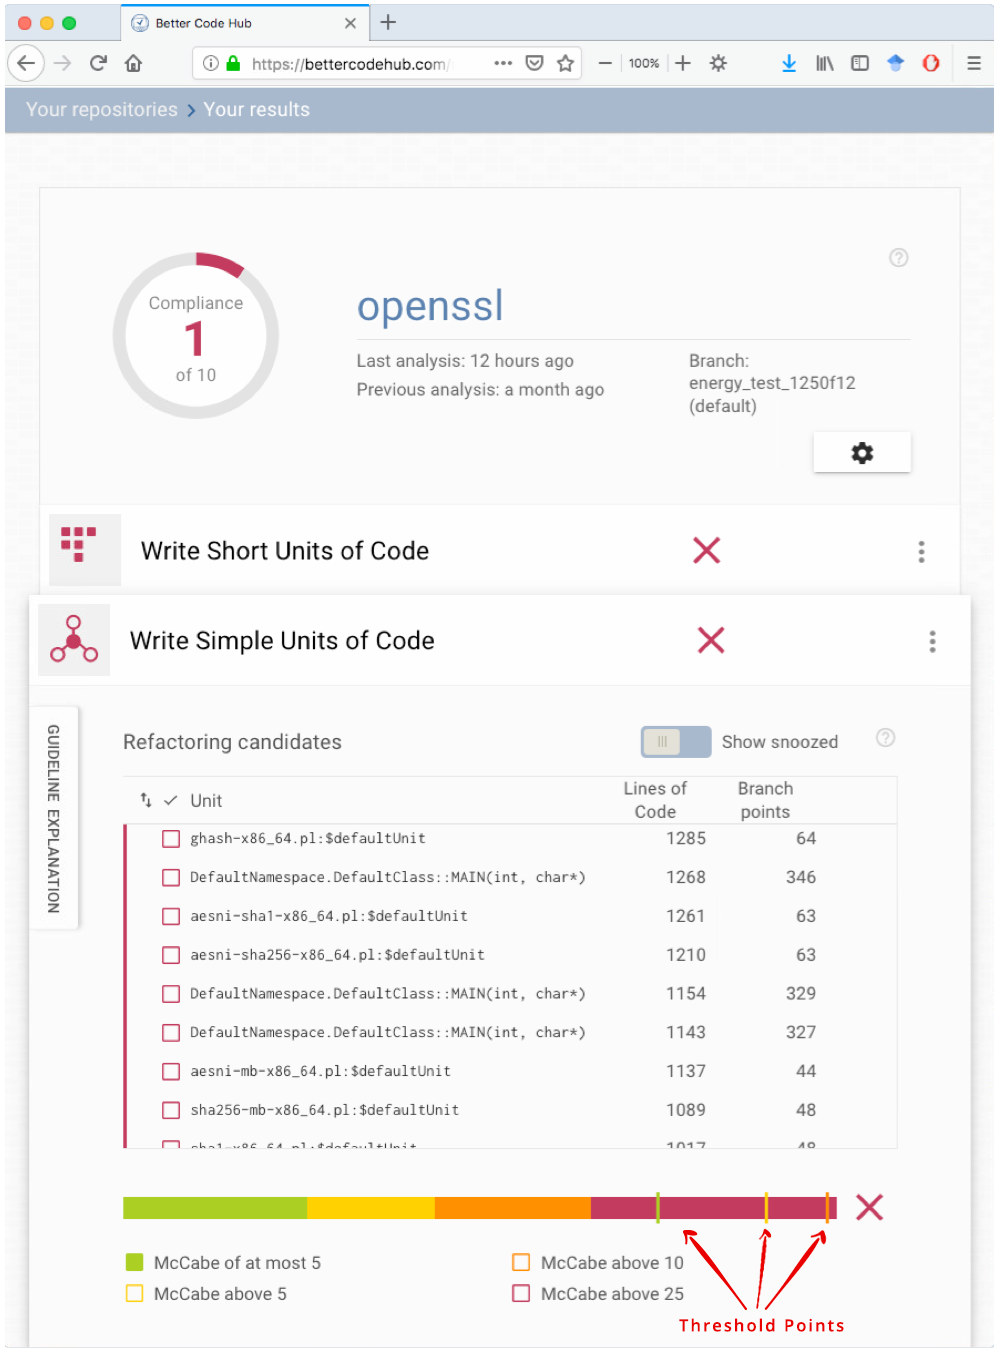
\includegraphics[width=0.45\textwidth]{figures/bch_report.png}
 	\caption{Maintainability report of OpenSSL CVE-2014-3506 vulnerability
refactoring for the guideline \emph{Write Simple Units of Code} provided by
\emph{Better Code Hub}. This version of OpenSSL does not comply with the
guideline in the example since the bars do not reach the threshold points. This
example only complies with $\frac{1}{10}$ guidelines (\emph{Write Clean Code}).}
	\label{fig:bchrep}
\end{figure}

\emph{Units} are the smallest groups of code that can be maintained and executed
independently \cite{Visser:2016:OREILLY}. McCabe \cite{1702388} is a software
metric that calculates the number of linearly independent paths of the source
code. BCH uses this metric to measure the number of branch points in the
\emph{Write Simple Units of Code} guideline. The bar represents the top 30 of
units that violates the guideline, sorted by severity, which is indicated by the
colors of the checkboxes. The green bar represents the number of compliant
branch points per unit (\emph{at most 5}), i.e., the units are compliant with
ISO 25010 \cite{iso:2011}. Yellow, orange and red bars represent units that do
not comply with medium (\emph{above 5}), high (\emph{above 10}) and very high
(\emph{above 25}) severity levels. In the bar, there are marks that pinpoint the
compliance thresholds for each severity level. \Sof{@todo: Adress thresholds confusion}

\begin{figure}[h]
 	\centering 	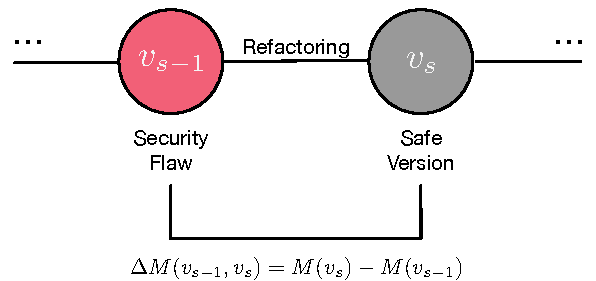
\includegraphics[width=0.49\textwidth]{figures/commit.pdf}
 	\caption{Maintainability difference for security commits}
	\label{fig:commit}
\end{figure}

Aiming to analyze the impact of security refactorings, we use BCH to compute
maintainability of two different versions of the project (Figure
\ref{fig:commit}):
\begin{itemize}
	\item $v_{s-1}$, the version containing the security flaw, i.e., before the
	refactoring;
	\item $v_{s}$, the version after fixing the security flaw, i.e., after the
	refactoring;
\end{itemize}

The BCH tool does not compute the final score that our study needs to compare
maintainability amongst different project versions. Thus, our work proposes an
equation to capture the distance between the current state of the project and
the standard thresholds based on previous work \cite{Olivari:2018}.
\begin{itemize}
	\item \textbf{Size project changes do not affect the maintainability
	difference between two versions, $\Delta M (v_{s-1},v_{s})$.} In this work, we
	aim to evaluate the alike security patterns occurring in different projects.
	Thus, normalization based on its size cannot be used - we convert relative
	data to the respective number of lines of code.
	\item \textbf{Distance to lower severity levels are less penalized than to the
	thresholds in high severity levels.} Severity level weights based on the
	severity level to count lines of code that violate maintainability guidelines.
\end{itemize}

We compute the mean average of the maintainability score $M(v)$ for all the
selected guidelines, as follows:



\begin{equation}
    M(v) = \sum_{g \in G}^{} M_{g}(v)
\end{equation}

\noindent
where $G$ is the group of selected maintainability guidelines from BCH (Table
\ref{tab:guidelines}) and $v$ is the version of the software under evaluation.
The maintenance $M$ based on the guideline $g$ for a given version of a project
is computed with the following equation:

\begin{equation}
    M_{g} = \frac{1}{|L|} \sum_{l \in L}^{} C(l) , L = \{medium, high, veryHigh\}
\end{equation}

\noindent
where $C$ is the compliance with the maintainability guideline for the given
severity level (medium, high, and very high) and $L$ is the group of severity
levels of maintainability infractions. The compliance $C$ for a given severity
level $l$ is derived by:

\begin{equation}\label{eq:3}
    C(l) = LOC_{compliant}(l) - w(l) * LOC_{\neg compliant}(l)
\end{equation}

\noindent
where $LOC_{compliant}(l)$ are the lines of code that comply with the guideline
at the given severity level $l$, $LOC_{\neg compliant}(l)$ are the lines of code
that do not comply with the guideline at the given severity level $l$ and $w(l)$
is the weight factor to boost the impact of non-compliant lines in comparison to
compliant lines. Finally, the term $w(l)$ is calculated as follows:

\begin{equation}
    w(l) = \frac{1 - T(l)}{T(l)}
\end{equation}

\noindent
where $T(l)$ is the threshold in percentage of the lines of code that are
accepted to be non-compliant with the guideline for the severity level $l$. This
is a standard value defined by BCH. In other words, the factor $w$ is used in
Equation \ref{eq:3} to highlight the lines of code that are not complying with
the guideline. Then, we compute the difference of maintainability between the
security commit ($v_{s}$) and its parent commit ($v_{s-1}$), as illustrated in
Figure \ref{fig:commit}.

\subsection{Statistical Validation}\label{sec:statsval}
%
To validate the maintainability differences in different groups of commits
(e.g., baseline and security commits), we use the Paired Wilcoxon signed-rank
test with the significance level $\alpha = 0.05$ \cite{10.2307/3001968} . In
other words, we test the null hypothesis that the maintainability difference
between pairs of versions $v_{v-1}$, $v_v$ (i.e., before and after a
security-commit) follows a symmetric distribution around $0$. However, when the
difference between groups is zero, the observations are discarded. Thus, we use
a more robust approach of the wilcoxon test, the Wilcoxon test by Pratt which
provides an alternative that incorporates the cases where the maintainability
difference is zero \cite{10.2307/2282543}. To understand the effect-size, as
advocated by the Common-language effect sizes \cite{graw:1992}, we compute the
mean difference, the median of the difference, and the percentage of cases that
reduce maintainability.
%
\section{Results}\label{sec:results}

In total, this study evaluates $607$ security and baseline commits from 94 
different open-source projects distributed among 5 different main types of 
software, Figure \ref{fig:domain}. The following section presents the results 
obtained for each research question.

\begin{framed}
\textit{\textbf{RQ1} What is the impact of security refactorings on the 
maintainability of open-source software?}
\end{framed}


The impact of security and baseline commits in the maintainability of 
open-source software is presented in Figure \ref{fig:secvsreg}. For each type 
of change, three types of impact of refactorings in the software maintainability 
are presented: \emph{negative}, maintainability decreases (\emph{red}); \emph{none}, 
maintainability stays the same (\emph{yellow}); and, \emph{positive}, maintainability 
increases (\emph{green}). In front of each group, it is presented the mean ($\overline{x}$) 
and median ({$\widetilde{x}$) of the maintainability difference and the p-value 
resulting from the Wilcoxon signed-rank test.

\begin{figure}[h]
 	\centering 	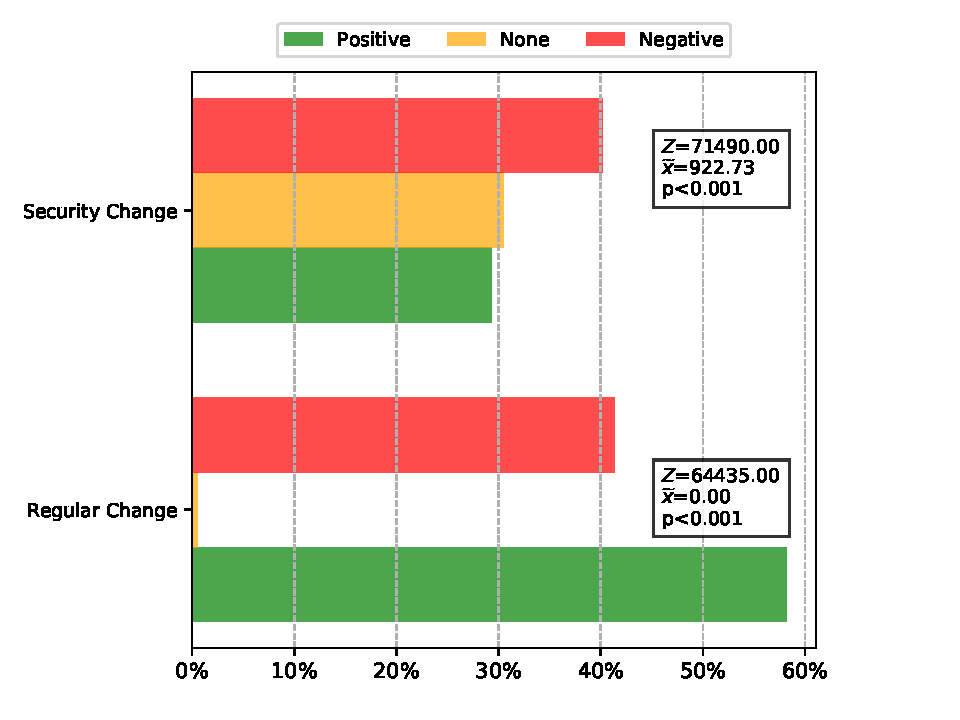
\includegraphics[width=0.5\textwidth]{figures/maintainability.pdf}
 	\caption{Maintainability difference for security and baseline refactorings}
	\label{fig:secvsreg}
\end{figure}

Regarding security commits results, we observe that maintainability decreases 
in 40.20\% (244), stays equal in 30.5\% (185) and increases in 29.33\% (178)  
of the cases after security refactorings being applied. The resulting p-value 
of the Wilcoxon signed-rank test is $1.21$x$10^{-10}$. Since the p-value is below 
the significance level of $0.05$, it is reasonable to affirm that \emph{security 
refactorings have a negative impact in the maintainability of open-source software}.

For regular commits, we also observe that maintainability decreases in 41.35\% 
(251) of the cases after regular refactorings being applyed. But in contrast 
to security commits, it increases in 58.16\% (353) and stays equal in 0.5\% 
(3) of the cases. The resulting p-value of the Wilcoxon signed-rank test is 
$1.54$x$10^{-6}$. Since the p-value is below the significance level of $0.05$, 
it is reasonable to affirm that \emph{regular refactorings have a positive 
impact in the maintainability of open-source software}.

\begin{figure}[h]
 	\centering
 	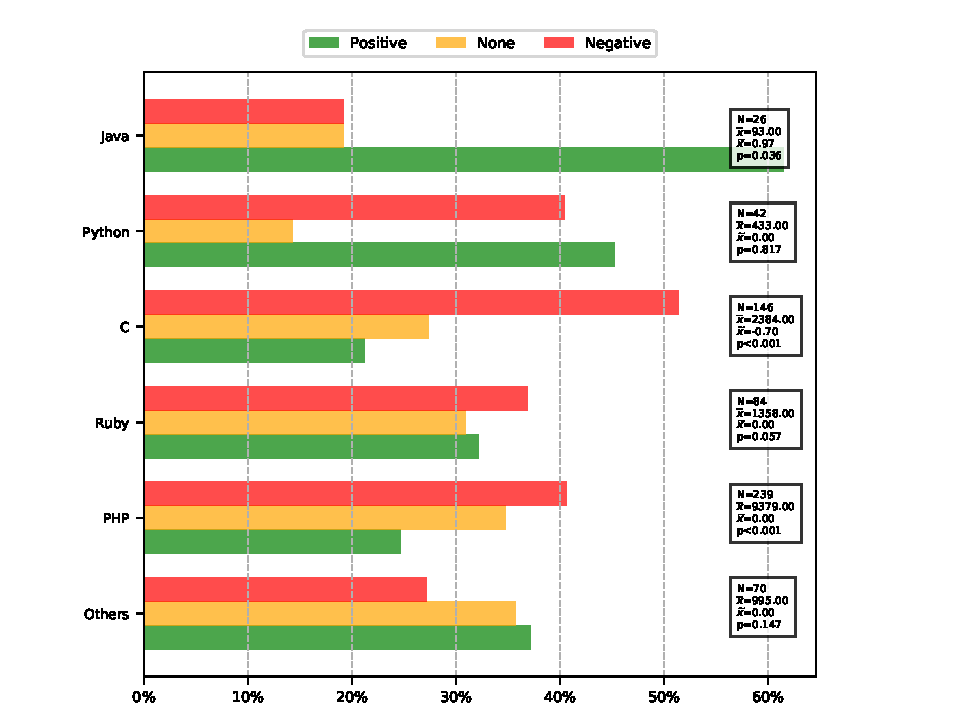
\includegraphics[width=0.55\textwidth]{figures/language.pdf}
 	\caption{Maintainability difference by language after security refactorings}
	\label{fig:lang_main}
\end{figure}

In this study, we also evaluated the impact of each programming language on the 
maintainability of open-source software, Figure \ref{fig:lang_main}. Although the
dataset contains security refactorings for more than $13$ languages, we only
present the results for \emph{Java}, \emph{C}, \emph{Ruby} and \emph{PHP} because
one of the requirements of the Wilcoxon signed-rank test is that the input sample
has to have more than $20$ measurements. The other languages were integrated in the
\emph{Others} set. The results of the Wilcoxon signed-rank test by pattern returned 
statistical evidence which supports that the maintainability of open-source software 
decreases for security refactorings in 3 different languages: \emph{C} 
(p = $5.72$x$10^{-9}$), Ruby (p = 0.057) and PHP (p = $3.54$x$10^{-6}$). The results 
also provide statistical significance for when security refactorings are performed
in \emph{Java} (p = $3.61$x$10^{-2}$). \emph{Python} and the other languages 
that integrate the \emph{Others} set contain more cases where the maintainability
increases. However, the results obtained for these patterns are not statistically 
significant.



\begin{framed}
\textit{\textbf{RQ2} Which patterns of security refactorings are more likely to 
affect open-source software maintainability?}
\end{framed}

The impact of each type of security refactoring on the maintainability of 
open-source software is presented in Figure \ref{fig:pat}. The results of the 
Wilcoxon signed-rank test by pattern returned statistical evidence which 
supports that the maintainability of open-source software decreases for 4 
different patterns: Broken Autentication (p = 0.018), Denial-of-Service 
(p = 0.029), Memory Leak (p = 0.009) and Miscellaneous (p = $3.07$x$10^{-4}$). 
The results also returned statistical significance that evidence that maintainability
is more likely to not suffer differences for open-source software after removing 
Components with Known Vulnerabilities (p = $7.96$x$10^{-4}$) and fixing Cross-Site 
Scripting Vulnerabilities (p = 0.001). Injection and Cross-Site Request Forgery 
produced more cases where the refactorings had a negative impact in the maintainability. 
However, the results obtained for these patterns are not statistically significant.

Projects with Broken Authentication flaws are the most affected ones by security 
refactorings. 55.3\% (21) of the refactorings had a negative impact in the maintainability 
while 35\% (11) had a positive impact and only 13.8\% (6) did not suffer any 
change. The results also show that fixing memory leaks affects the maintainability
of 51.3\% (41) of the cases and leaves only 13.8\% (11) of the cases unaffected. 
In 35\% (28) of the cases, maintainability increased. Refactoring vulnerabilities 
that allow denial-of-service attacks (e.g., CVE-2014-3506) has a negative impact 
of 47.5\% (19) in the maintainability of open-source software. 30.0\% (12) of 
the cases exhibit maintainability improvement while 22.5\% (9) show that overall 
maintainability does not suffer any change. Miscellaneous refactorings pattern 
integrates several types of security flaws whose impact is of 43.1\% (84) negative 
in the maintainability of open-source sofware. 31.8\% (62) of the cases do not 
exhibit any change in maintainability and 25.1\% (49) of cases have a positive 
impact on the maintainability of open-source software.

It is also important to notice that overall the maintainability of open-source 
software is not affected by Cross-Site Scripting vulnerabilities and by Using 
Components with Know Vulnerabilities. Cross-Site Scripting does not suffer any 
decrease in the maintainability of 55.3\% (63) of cases and 21.1\% (24) have a 
positive effect on it. Only 23.7\% (27) of the cases hinder the software 
maintainability. From 21 cases evaluated for Using Componentes with Known 
Vulnerabilities, only 4.8\% (1) has a positive effect in the maintainability 
of software. 14.3\% (3) harms maintainability software and 81\% has no effect 
in the maintainability.

\begin{figure}[h]
 	\centering
 	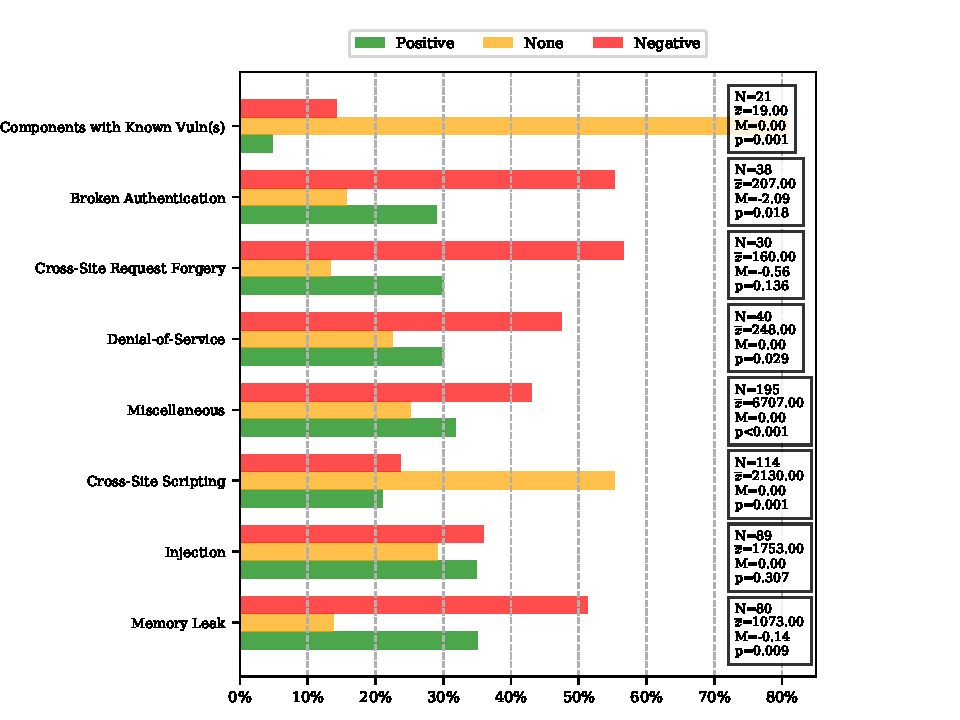
\includegraphics[width=0.55\textwidth]{figures/category.pdf}
 	\caption{Maintainability difference by pattern after security refactorings}
	\label{fig:pat}
\end{figure}

\section{Discussion}\label{sec:discussion}

In this section, we discuss the results and answer the proposed research questions.

\begin{framed}
\textit{\textbf{RQ1} What is the impact of security refactorings on the maintainability 
of open-source software?}
\end{framed}

\textbf{\textit{Security refactorings harm the maintainability of open-source software.}}

40.2\% of the security refactoring have a negative impact on the maintainability 
of open-source software, Figure \ref{fig:secvsreg}. This raises a new tradeoff when
developers need to fix vulnerabilities on their projects because they might be affecting 
the software maintainability or even introducing new vulnerabilities. This study exhibits
proof that developers may have to reduce maintainability for the sake of safety. We understand 
that developers should be able to produce secure code without affecting the maintainability of 
their projects. But there are still some concerns that need to be addressed: 
\begin{itemize}
	\item \textbf{Security Frameworks} need to be secure. Unfortunately, there are several 
	vulnerabilities that stay undisclosed. Thus, developers should not trust them blindly and 
	check defaults.
	\item \textbf{Documentation} of software should provide developers with the best practices to implement safe and maintainable software. Unmaintainable code is difficult to test, analyze and re-use.
	\item \textbf{Proper Authorization Mechanisms} should be designed and implemented. This is
	one of the most complex security features to implement. Some mechanisms might assist authorization maintenance in long run, such as the combination of \texttt{HTTP} filters with \texttt{Spring Security} annotations.
	\item \textbf{Deprecated code} should be avoided by developers. They should integrate tools such as BCH on their projects CI/CD pipelines to help them be more aware of the maintainability of their code and issues (e.g., dead and duplicated code). 
	\item\textbf{Programming Languages} should provide new mechanisms to easily implement security patterns without endangering maintainability.
	
\end{itemize}

	

We would expect that the negative impact of programming languages on maintainability 
would be more intense due to the buzz of the last years surrounding the idea that 
poor design of programming languages and lack of using the best practices lead to 
more buggy and vulnerable code~\cite{Ray:2017:LSP:3144574.3126905, 2019arXiv190110220B}. 
However, Figure \ref{fig:lang_main} shows that only \emph{C} has a negative impact of more than 50\% on 
software maintainability. We suspect that these values are the result of projects 
contributions policies. 9 out of 10 projects --- the equivalent to 31.8\% of the commits --- 
of the top-10 of dataset projects with more contributors have restrict contribution 
policies regarding code standards. Some examples are the \texttt{laravel/framework}, 
\texttt{php/php-src}, \texttt{openssl/openssl} and 
\texttt{cakephp/cakephp}. For instance, \texttt{laravel/framework} requires the 
\texttt{PSR-2 Standard}\footnote{PSR-2 Standard available at 
https://www.php-fig.org/psr/psr-2/ (Accessed on \today{}}).


\begin{framed}
\textit{\textbf{RQ2} Which patterns of security refactorings are more likely to affect open-source software maintainability?}
\end{framed}

\textbf{\textit{Broken Authentication \& Session Management, Denial-of-Service attacks and Memory Leaks and Miscellaneous patterns are more likely to affect open-source software maintainability.}} Although there are
a few refactorings that harm software maintainability in the \emph{Cross-Site Scripting} and \emph{Using 
Components with Know Vulnerabilities}, overall maintainability does not suffer any changes for these patterns.
For the remaining patterns, \emph{Injection} and \emph{Cross-Site Request Forgery}, results are not statistically
significant.

The impact of a refactoring depends on its complexity, i.e., if the refactoring adds complexity to the codebase it is probably affecting the software maintainability. One evidence of that is the fact of \emph{Cross-Site Scripting} and \emph{Using Components with Know Vulnerabilities} refactorings endure more cases without any impact in the maintainability. Typically, these type of vulnerabilities are one line fixes --- adding an \texttt{escape} function or changing the version of the component, respectively. Whereas, Broken Authentication and vulnerabilities such as the one presented in Section \ref{sec:motivation} responsible by DoS attacks are more difficult to fix (several code lines deleted and added). Another example is the Apple authentication flaw discovered in 2017 (CVE-2017-13872)\footnote{CVE-2017-13872 details available at https://support.apple.com/en-us/HT208315 (Accessed on \today{}}, where any user could login as root with an empty password. Patrick Wardle examined the cause of the issue\footnote{\emph{Why $<$blank$>$ Gets You Root} available at https://objective-see.com/blog/blog\_0x24.html (Accessed on \today{}} and conclude that the flaw was due to the introduction of high cyclomatic complexity in a method used to verify the password. In sum, \emph{Cross-Site Scripting} and \emph{Using Components with Known Vulnerabilities} should take part of the developers preocupations along with the other patterns that explicitly hinder maintainability because despite their low complexity these are patterns that still produce a considerable negative impact on the maintainability. Real efforts have been made in creating and incorporating coding standards and best practices in software production. However, security is still far from perfection and fixing vulnerabilities might hinder software maintainability. Thus, it is important to provide tool support to developers to help them applying these patterns without harming software maintainability.


\section{Threats to Validity}\label{sec:threats}
%
The following section presents the potential threats to validity of this study.
%
\subsection{Construct}
%
The maintainability formula was inferred based on the reports of the Better Code Hub.
Since the dataset has a broad group of open-source projects with different backgrounds, this metric may not be suitable for all of them. \Sof{Improve it} However, BCH does have a representative benchmark of
closed and open-source software projects that is under the calculation of the thresholds used in the computation of each maintainability guideline (Table \ref{tab:guidelines})~\cite{Visser:2016:OREILLY, Baggen2012}.

\subsection{Internal}

The security refactorings dataset provided by the previous
work~\cite{Reis:2017:IJSSE} was collected based on the messages of GitHub commits produced by
project developers to classify the changes perfomed by them to fix security flaws. This approach discards security refactorings that were not explicit in commits messages.

Baseline commits are retrieved randomly by selecting one commit from the same project of a given security refactoring. This approach softens the differences that may result from the
characteristics of each project. However, maintainability still may be affected by the developers experience, coding style and software contribution polices. But maintainability difference is not evaluated at this level.

\subsection{External}

In contrast to the BCH benchmark, this study uses a dataset that only covers open-source software to perform the maintanibility evaluation. Thus, answering these questions to closed commercial applications may be a future work opportunity.

All the security commits are described in English. This approach discards security refactorings provided in other languages.

\section{Related Work}\label{sec:rw}

\subsection{Security Maintainability Models}

~\cite{6616351,oswap:2009,common:2009}




\section{Conclusion and Future Work}\label{sec:conclusions}

This work presents an empirical study on the impact of 607 security refactorings on
the maintainability of 94 open-source projects. We leveraged Better Code Hub reports
of each project version to calculate maintainability based on a model proposed in 
previous work.

Security refactorings significantly affect the software maintainability of open-source 
software, i.e., developers hinder maintainability when fixing vulnerabilities. We found
this evidence in 40.2\% of the studied cases. Regarding regular commits, it seems that
overall maintainability increases (50.16\%). However, there is still a very considerable amout of
cases that harm maintaniability (41.35\%). This study also exhibits evidence that some patterns
need more attention than others. Broken Autentication issues, Denial-of-Service attacks 
and Memory Leaks endure maintainability in 55.3\%, 51.3\% and 47.5\%, respectively.

Following the implications of our work, we draw attention for the need of secure security frameworks,
code best practices documentation to produce safe and maintainable code, proper authorization 
mechanisms design and implementation, better tools to introduce in the CI/CD pipeline to help software
maintenance and new or improved programming languages to allow developers to easily implement safety in
their software without endangering maintainability.

As future work, this study may be extended in many directions such as analyze which guidelines are
more likely to affect security refactorings; evaluate the impact of programming languages of the
maintainability of each refactoring pattern; investigate if there is any correlation between 
software maintainability and projects popularity; expand our methodology with other software quality
properties; and, validate these findings with closed or private software. 


\section*{Acknowledgment}\label{sec:ack}

\noindent
We thank to the Software Improvement Group (SIG) team for all the support and
help in validating our methodology.

\balance

{
 \bibliographystyle{IEEEtran}
  \bibliography{icpc19}
}

\end{document}
